\documentclass[pdf, intlimits, 12pt, unicode]{beamer} %Для Latex2Pdf  tex -> pdf

%Пакеты для русского языка
\usepackage[T2A]{fontenc}
\usepackage[utf8]{inputenc}
\usepackage[english,russian]{babel}

%Пакет для вставки рисунков
\usepackage{graphicx}
%AMS TEX значки и пр.
\usepackage{amssymb}
\usepackage{amsthm}
\usepackage{amssymb, amsmath, amsthm, amsfonts, amscd, geometry}


%Привычный шрифт для математических формул
\usefonttheme[onlymath]{serif}

%Нужно включать, если используется "тема" (стиль оформления) по умолчанию
\usepackage{beamerthemesplit}

%Общий стиль ("тема") оформления слайдов
%Требование: черные буквы на белом фоне
\usetheme{Warsaw}

\addtobeamertemplate{navigation symbols}{}{%
    \usebeamerfont{footline}%
    \usebeamercolor[fg]{footline}%
    \hspace{1em}%
    \insertframenumber/\inserttotalframenumber
}
\setbeamercolor{footline}{fg=black}
\setbeamerfont{footline}{series=\bfseries}

%Более крупный шрифт для подзаголовков титульного листа
\setbeamerfont{institute}{size={\fontsize{13}{16}}}
\setbeamerfont{frametitle}{size={\fontsize{16}{19}}}

%Задание команды (\bluetext) для выделения конкретным (синим) цветом
%(используйте \alert для выделения цветом выбранной "темы")
%\setbeamercolor{bluetext_color}{fg=blue}
%\newcommand{\bluetext}[1]{{\usebeamercolor[fg]{bluetext_color}#1}}


\newcommand{\Expect}{\mathbb E}
\newcommand{\PRob}{\mathbb P}
\newcommand{\leqs}{\leqslant}
\newcommand{\geqs}{\geqslant}
\newcommand{\eps}{\varepsilon}
\DeclareMathOperator{\re}{Re}
\DeclareMathOperator{\I}{I}


\newtheorem*{theoremm}{Теорема}
\newtheorem*{lemmaa}{Лемма}
\newtheorem*{notee}{Замечание}




%Если используется последовательное появление пунктов списков на слайде
%(не злоупотребляйте в слайдах для защиты дипломной работы), чтобы
%еще непоявившиеся пункты были все-таки немножко видны.
%\setbeamercovered{transparent}

\title{Рост двудольных графов с~рёберным приоритетом}
\author{Ерохин Станислав Евгеньевич, гр. 512}
\institute{
	\vspace{0.30cm}\\
    Научный руководитель: к.ф.-м.н., д. Якубович~Ю.~В. \\
    Рецензент: к.ф.-м.н., д. Валландер С.\,С. \\
}
\date{
}

\begin{document}

\begin{frame}
    \titlepage
\end{frame}

\begin{frame}
    \frametitle{BitTorrent}
    Протокол для кооперативного обмена файлами через интернет -- BitTorrent:
    \begin{itemize}
        \item создан в 2001 году,
        \item сейчас более 30\% трафика.
    \end{itemize}
    \medskip
    \medskip
    
    Отличительные оссобенности:
    \begin{itemize}
		\item файл делится на фрагменты,
		\item клиенты обмениваются фрагментами;
		\item изначально файл только у одного клиента.
    \end{itemize} 
\end{frame}

\begin{frame}
	\frametitle{Двудольный граф и BitTorrent}
	\begin{figure}[t]
		\vspace*{-0.43in}
		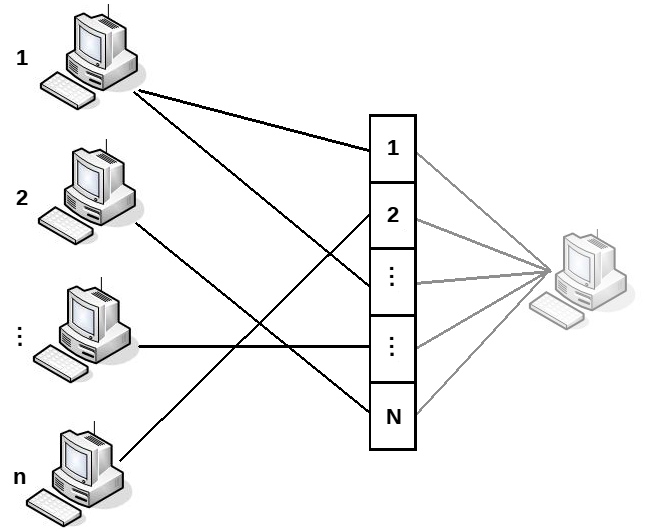
\includegraphics[scale=0.4]{clients}
		\vspace*{-0.2in}
	\end{figure}
	Доли: клиенты и фрагменты. 
	Ребра: наличие фрагмента. \\
	Клиент, у которого есть все фрагменты --- не участвует.\\ 
	Модель кодирует, как выбираются фрагменты.\\
	
\end{frame}

\begin{frame}
	\frametitle{Двудольный граф и BitTorrent}
	Следим за минимальной степенью фрагмента: $Q(G)$.\\
	
	Почему именно за ней:
	\begin{itemize}
		\item если $Q(G)$ достаточно большая, то мала вероятность "потерять" файл;
		\item влияет на характер обмена фрагментами между клиентами.
	\end{itemize}
	Хотим познать такой момент $m$, что $Q(G_m) \geqs q$.
\end{frame}


\begin{frame}
	\frametitle{обозначения}
	$G_m$ --- граф на шагу $m$. \\
	$n$ --- количество клиентов. \\
	$N$ --- количество фрагментов. \\
\end{frame}

\begin{frame}
	\frametitle{Модели}
	Было рассмотрено 3 модели:
	\begin{itemize}
		\item Равномерный выбор рёбер.
		\item Выбор клиента, затем выбор ребра.
		\item Выбор клиента, ребро к редкому фрагменту.
	\end{itemize}
\end{frame}



\begin{frame}
\begin{theoremm}[Для первой модели]
Пусть $q, \sigma \in (0, 1)$. Возьмем 
\begin{align*}
& m = \min(nN, \lceil pnN + 2\sqrt{pnN} \rceil), \quad \text{ где} \\
& p \geqs q + c + \sqrt{c^2+2qc}, \quad c = \frac{\ln(2N) - \ln(\sigma)}{n}.
\end{align*}
Тогда в графе $G_m$ с вероятностью, большей, чем $1 - \sigma$, все фрагменты будут скачены хотя бы $qn$ клиентами:
\begin{equation*}
\PRob\big(Q(G_m) \geqs qn\big) > 1 - \sigma.
\end{equation*}
\end{theoremm}

\begin{theoremm}[Для второй модели]
Если $(q+c) < \frac{1}{4}$, то неравенство на $p$ заменяется на:
\begin{equation*}
p \geqs 2\left(q + c + \exp\left(-\frac{N}{18}\right) \right).
\end{equation*}

\end{theoremm}
\end{frame}

\begin{frame}

\begin{lemmaa} \label{l1}
Пусть $A$ --- множество всех графов, которые обладают некоторым монотонным свойством, а $\delta \in (0,1)$.
Тогда, если $\PRob( H_p \in A) \geqs 1 - \eps$, то
\begin{equation*} \label{l1_1}
\PRob(G_{\lceil pnN(1+\delta) \rceil} \in A) > 1 - \frac{\eps}{1 - \exp\left(-\frac{\delta^2}{4}pnN\right)},
\end{equation*}
a если $\PRob( H_p \in A) \leqs \eps$, то
\begin{equation*}\label{l1_2}
\PRob(G_{\lfloor pnN(1-\delta) \rfloor} \in A) < \frac{\eps}{1 - \exp\left(-\frac{\delta^2}{2}pnN\right)}.
\end{equation*}
\end{lemmaa}

\end{frame}

\begin{frame}	
	\begin{theoremm}
		Пусть $q \in [0, \frac{1}{5} - \frac{2}{n}]$. 
		Возьмём $m \geqs (qn + 2) N$, тогда в графе $G_m$ с~вероятностью большей, чем 
		$1 - n\exp\left(-\frac{N}{5}\right) +  \exp\left(- \frac{N}{20}\right)$, все фрагменты скачены как минимум $qn$ клиентами:
		\begin{equation}
		\PRob\Big( Q(G_m) \geqs qn \Big) > 1 - n\exp\left(-\frac{N}{5}\right) +  \exp\left(- \frac{N}{20}\right).
		\end{equation}
	\end{theoremm}

\begin{notee}
Пусть $q \in [0,1]$. Тогда, если мы возьмём $m < qnN$, то в любом графе $G$, в котором ровно $m$ ребер, точно будет фрагмент, 
со степенью меньшей $qn$, т.е. $Q(G) < qn$.
\end{notee}

\end{frame}


\end{document}
